\documentclass[10pt]{article}
\usepackage[polish]{babel}
\usepackage[utf8]{inputenc}
\usepackage[T1]{fontenc}
\usepackage{graphicx}
\usepackage[export]{adjustbox}
\graphicspath{ {./images/} }
\usepackage{amsmath}
\usepackage{amsfonts}
\usepackage{amssymb}
\usepackage[version=4]{mhchem}
\usepackage{stmaryrd}

\title{VIII Konkurs matematyczny St@ś }

\author{}
\date{}


\begin{document}
\maketitle
XIV LO im. Stanisława Staszica\\
2 czerwca 2008 roku\\
klasa V\\
Na rozwiazanie poniższych zadań masz 90 minut.\\
Kolejność rozwiqzywania tych zadań jest dowolna.\\
Wszystkie zadania sa jednakowo punktowane.\\
Maksymalna liczbę punktów może uzyskać jedynie petne rozwiqzanie, z uzasadnieniem i odpowiedzia.\\
Uzywanie korektora i korzystanie z kalkulatora jest niedozwolone.

\section*{Zadanie 1.}
W każdą kratkę wpisz taką cyfrę, aby poniższe dodawanie ułamków było prawdziwe. (W różne kratki możesz wpisać różne cyfry.)\\
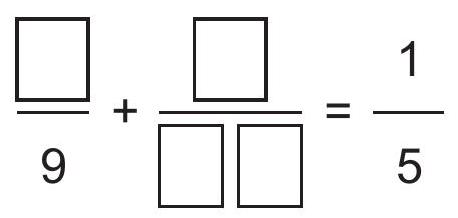
\includegraphics[max width=\textwidth, center]{2024_11_21_a60e976091171712aedfg-1(1)}

\section*{Zadanie 2.}
Dany jest trójkąt \(A B C\), w którym \(|A B|=|B C|=2008\).\\
Na bokach \(A B, B C, C A\) leżą takie punkty \(K, L, M\), że czworokąt \(K B L M\) jest równoległobokiem (jak na rysunku obok).\\
Oblicz obwód tego równoległoboku.\\
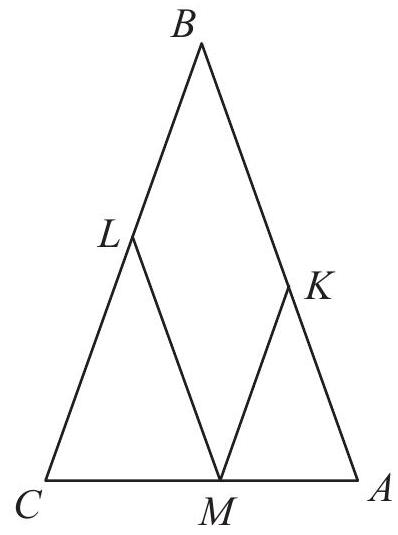
\includegraphics[max width=\textwidth, center]{2024_11_21_a60e976091171712aedfg-1(2)}

\section*{Zadanie 3.}
Podaj przykład takiej liczby pięciocyfrowej, której suma cyfr jest równa 4, i która jest kwadratem liczby naturalnej. Podaj jeszcze dwa inne przykłady takich liczb.\\
Uzasadnij, że Twoje przykłady są prawidłowe.

\section*{Zadanie 4.}
Podaj wymiary takiego prostopadłościanu, w którym suma pól pewnych dwóch ścian jest większa od sumy pól pozostałych ścian. Uzasadnij, że podany przykład jest prawidłowy.

\section*{Zadanie 5.}
Z ośmiu kart ułożono dwa dodawania poziomo i dwa dodawania pionowo. Na każdej karcie jest liczba naturalna, ale niektóre karty nie zostały odkryte. Znajdź liczbę na szarej karcie. Uzasadnij swoją odpowiedź.\\
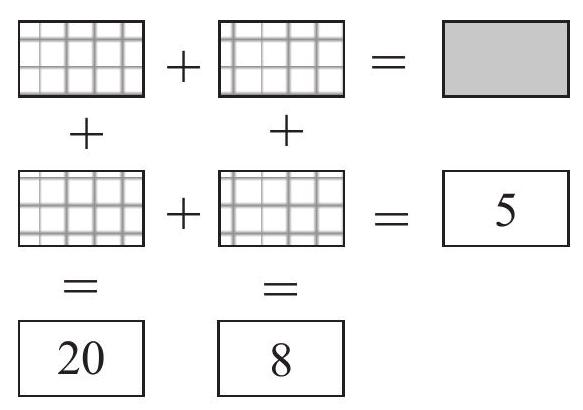
\includegraphics[max width=\textwidth, center]{2024_11_21_a60e976091171712aedfg-1}


\end{document}